\begin{figure}
\pgfplotsset{width=0.5\textwidth,height=0.5\textwidth}
\centering
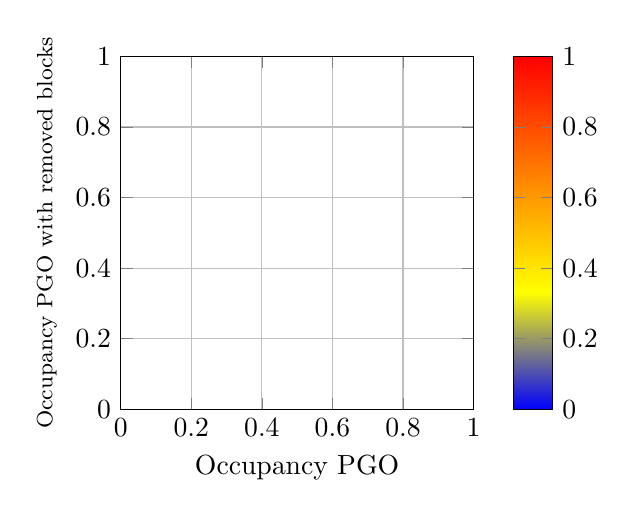
\begin{tikzpicture}
\begin{axis}[
	xlabel={Occupancy PGO},
	ylabel={\footnotesize Occupancy PGO with removed blocks},
	point meta min=0,
	grid=both,
	enlargelimits=false,
	colorbar,
	nodes near coords={\pgfmathprintnumber\pgfplotspointmeta},
	node near coords style={
		/utils/exec={\setbox0\hbox{\pgfmathprintnumber\pgfplotspointmeta}
		\pgfmathfloattomacro{\pgfplotspointmeta}{\F}{\M}{\E}
		\pgfmathsetmacro{\mycolor}{ifthenelse(\M*pow(10,\E)<100,"white","black")}
		},
		yshift=-7pt, color=\mycolor},
]

\runtex{register-occupancy}
\end{axis}
\end{tikzpicture}
\captionof{figure}{Occupancy based on vector register usage, when removing blocks}
\label{dia:registers_occupancy}
\end{figure}
